% Biên dịch bằng XeLaTeX (xelatex report.tex), chạy hai lần để cập nhật tham chiếu.
% Đặt được ở hai cách: biên dịch trong thư mục reports/, hoặc trên Overleaf với gốc dự án là customer_segmentation/
% (khi đó đặt report.tex làm Main document).
% Mọi số liệu thực nghiệm được lấy từ generated/values.tex và generated/table_*.tex,
% do notebooks/customer_segmentation.ipynb sinh ra; không gõ tay số liệu trong tệp này.
\documentclass[11pt,a4paper]{article}

% Không dùng babel-vietnamese: gói này ép bảng mã T5 của pdfLaTeX, gây lỗi font với XeLaTeX.
\usepackage{fontspec}
\usepackage[margin=2.2cm]{geometry}
\usepackage{graphicx}
\usepackage{adjustbox}
\usepackage{booktabs}
\usepackage{float}
\usepackage{caption}
\usepackage{enumitem}
\usepackage{amsmath}
\usepackage[hidelinks]{hyperref}

% Nạp font theo tên tệp (có sẵn trong TeX Live/Overleaf, đủ dấu tiếng Việt), không phụ thuộc fontconfig.
\setmainfont{texgyretermes}[
  Extension = .otf,
  UprightFont = *-regular,
  BoldFont = *-bold,
  ItalicFont = *-italic,
  BoldItalicFont = *-bolditalic]
\renewcommand{\figurename}{Hình}
\renewcommand{\tablename}{Bảng}
\setlength{\emergencystretch}{3em}
\graphicspath{{../figures/}{figures/}}
\setlist{itemsep=2pt, topsep=4pt}

% Tệp sinh tự động nằm ở generated/ (biên dịch trong reports/) hoặc reports/generated/ (gốc là customer_segmentation/).
\newcommand{\generated}[1]{\IfFileExists{generated/#1}{\input{generated/#1}}{\input{reports/generated/#1}}}
\generated{values.tex}

\title{Phân cụm khách hàng sàn thương mại điện tử\\
\large Bài thực nghiệm giữa kỳ — Phân tích và Khai phá dữ liệu}
\author{Mã sinh viên: 24022391 \\ Trường Đại học Công nghệ — ĐHQGHN}
\date{}

\begin{document}
\maketitle

\section*{Tổng quan}

Bài thực nghiệm xây dựng một quy trình phân cụm khách hàng hoàn chỉnh trên dữ liệu giả lập: sinh dữ liệu có cấu trúc tiềm ẩn, chủ động đưa vào các vấn đề chất lượng dữ liệu, phân tích, tiền xử lý, chuẩn bị đặc trưng, rồi so sánh K-Means trên dữ liệu chưa xử lý (nhánh A, baseline) và đã xử lý (nhánh B, processed).

Thông số theo mã sinh viên: $a=1$, $b=4$, $c=3$; $N=\NCustomers$ bản ghi; $\NInputFeatures$ thuộc tính đầu vào; tối thiểu 11 bản ghi ngoại lai. Toàn bộ mã nằm trong \texttt{notebooks/customer\_segmentation.ipynb}, dùng \texttt{np.random.default\_rng(42)} và \texttt{random\_state=42}. Notebook chạy tuần tự từ đầu đến cuối; mọi bảng và số liệu dưới đây được sinh tự động từ kết quả chạy.

%===========================================================================
\section{Câu a — Thiết kế và sinh dữ liệu}

\paragraph{Phương pháp.}
Dữ liệu gồm \NCustomers{} khách hàng, mỗi khách có \texttt{customer\_id} (không phải thuộc tính đầu vào) và \NInputFeatures{} thuộc tính: \texttt{tenure\_months}, \texttt{recency\_days}, \texttt{orders\_6m}, \texttt{total\_spend\_6m}, \texttt{avg\_order\_value}, \texttt{sessions\_30d}, \texttt{discount\_usage\_rate}, \texttt{return\_rate}, \texttt{category\_diversity}, \texttt{cart\_abandonment\_rate}, \texttt{favorite\_category} (8 mức), \texttt{preferred\_device} (3 mức). Đơn vị tiền là nghìn đồng.

Dữ liệu được sinh từ bốn nhóm hành vi tiềm ẩn: Loyal (\SegLoyal), Discount Seeker (\SegDiscount), Browser (\SegBrowser), Inactive (\SegInactive). Mỗi nhóm có tham số riêng:
\begin{itemize}
  \item số đơn: $1 + \text{Poisson}(\lambda)$;
  \item giá trị đơn trung bình: Lognormal;
  \item số phiên: Poisson với cường độ nhân hệ số Gamma (tức Negative Binomial);
  \item recency: Exponential với thang đo giảm khi số đơn tăng;
  \item các tỷ lệ: Beta;
  \item số danh mục: $1 + \text{Poisson}$, tối đa 8.
\end{itemize}

Các quy ước logic:
\begin{itemize}
  \item $\texttt{total\_spend\_6m} = \texttt{orders\_6m} \times \texttt{avg\_order\_value}$;
  \item mọi khách có ít nhất một đơn trong 6 tháng;
  \item $\texttt{recency\_days} \le 30 \times \texttt{tenure\_months}$;
  \item có mua trong 30 ngày thì có ít nhất một phiên truy cập.
\end{itemize}
Nhãn \texttt{true\_segment} chỉ lưu trong \texttt{metadata/simulation\_metadata.csv}.

Các vấn đề chất lượng dữ liệu được đưa vào theo thứ tự sau. Các bản ghi ngoại lai được chọn trước và không bị thêm nhiễu hay giá trị thiếu, để mỗi bản ghi ngoại lai chỉ mang đúng một loại lỗi.
\begin{itemize}
  \item \textbf{Ngoại lai:} \OutlierIds{} \texttt{customer\_id}, gồm \OutlierBusiness{} ngoại lai hợp lệ về nghiệp vụ (khách VIP có giá trị đơn gấp 4–6 lần; khách mua 60–80 đơn) và \OutlierError{} ngoại lai do lỗi dữ liệu (chi tiêu $\times 100$; \texttt{sessions\_30d}~$=999$; \texttt{return\_rate}~$=1.85$; \texttt{discount\_usage\_rate}~$=-0.40$; \texttt{tenure\_months}~$=-12$; \texttt{recency\_days}~$=-15$).
  \item \textbf{Nhiễu Gaussian}, mỗi biến trên \NoiseRecords{} bản ghi (40\%):
    \begin{itemize}
      \item \texttt{total\_spend\_6m}: nhiễu tương đối $x(1+\varepsilon)$, $\varepsilon \sim \mathcal{N}(0, 0.15^2)$;
      \item \texttt{sessions\_30d}: nhiễu cộng $\varepsilon \sim \mathcal{N}(0, \NoiseSessionsSd^2)$, với độ lệch chuẩn bằng $0.25$ lần độ lệch chuẩn của biến, làm tròn và cắt tại 0.
    \end{itemize}
  \item \textbf{Giá trị thiếu:}
    \begin{itemize}
      \item \texttt{avg\_order\_value}: MCAR, \MissAovCount{} ô (\MissAovPct\%);
      \item \texttt{cart\_abandonment\_rate}: MAR, \MissCartCount{} ô (\MissCartPct\%), xác suất thiếu tỷ lệ với $e^{-\texttt{sessions\_30d}/10}$.
    \end{itemize}
\end{itemize}

\paragraph{Lý do lựa chọn.}
Sinh theo nhóm tiềm ẩn tạo ra quan hệ hợp lý giữa các biến và cho phép kiểm chứng phân cụm bằng ARI. Phân phối Lognormal và Negative Binomial phù hợp với tiền tệ lệch phải và với biến đếm có phương sai lớn hơn trung bình. Nhiễu tương đối được dùng cho chi tiêu vì biến này trải từ vài trăm đến hàng chục nghìn: một độ lệch chuẩn tuyệt đối chung sẽ làm biến dạng mạnh khách chi tiêu thấp, thậm chí tạo giá trị âm. Cơ chế MAR được chọn vì khách ít truy cập có ít sự kiện giỏ hàng để ghi nhận.

\paragraph{Kết quả và nhận xét.}
Mọi điều kiện của đề bài được kiểm tra bằng \texttt{assert} và đều thỏa. Trung bình theo nhóm thay đổi đúng hướng thiết kế (Hình~\ref{fig:segments}), nhưng các nhóm chồng lấn: silhouette của nhãn giả lập trên \NNumericFeatures{} thuộc tính số đã chuẩn hóa chỉ là \TrueSilhouette.

Tác động của nhiễu:
\begin{itemize}
  \item chi tiêu thay đổi trung bình \NoiseSpendRelPct\%, tương quan trước/sau \NoiseSpendCorr;
  \item số phiên thay đổi trung bình \NoiseSessionsAbs{} phiên; \NoiseSessionsChanged/\NoiseRecords{} giá trị thực sự đổi, phần còn lại có nhiễu bị làm tròn về 0.
\end{itemize}
\UntouchedRecords{} bản ghi không chịu can thiệp nào.

\begin{figure}[H]
  \centering
  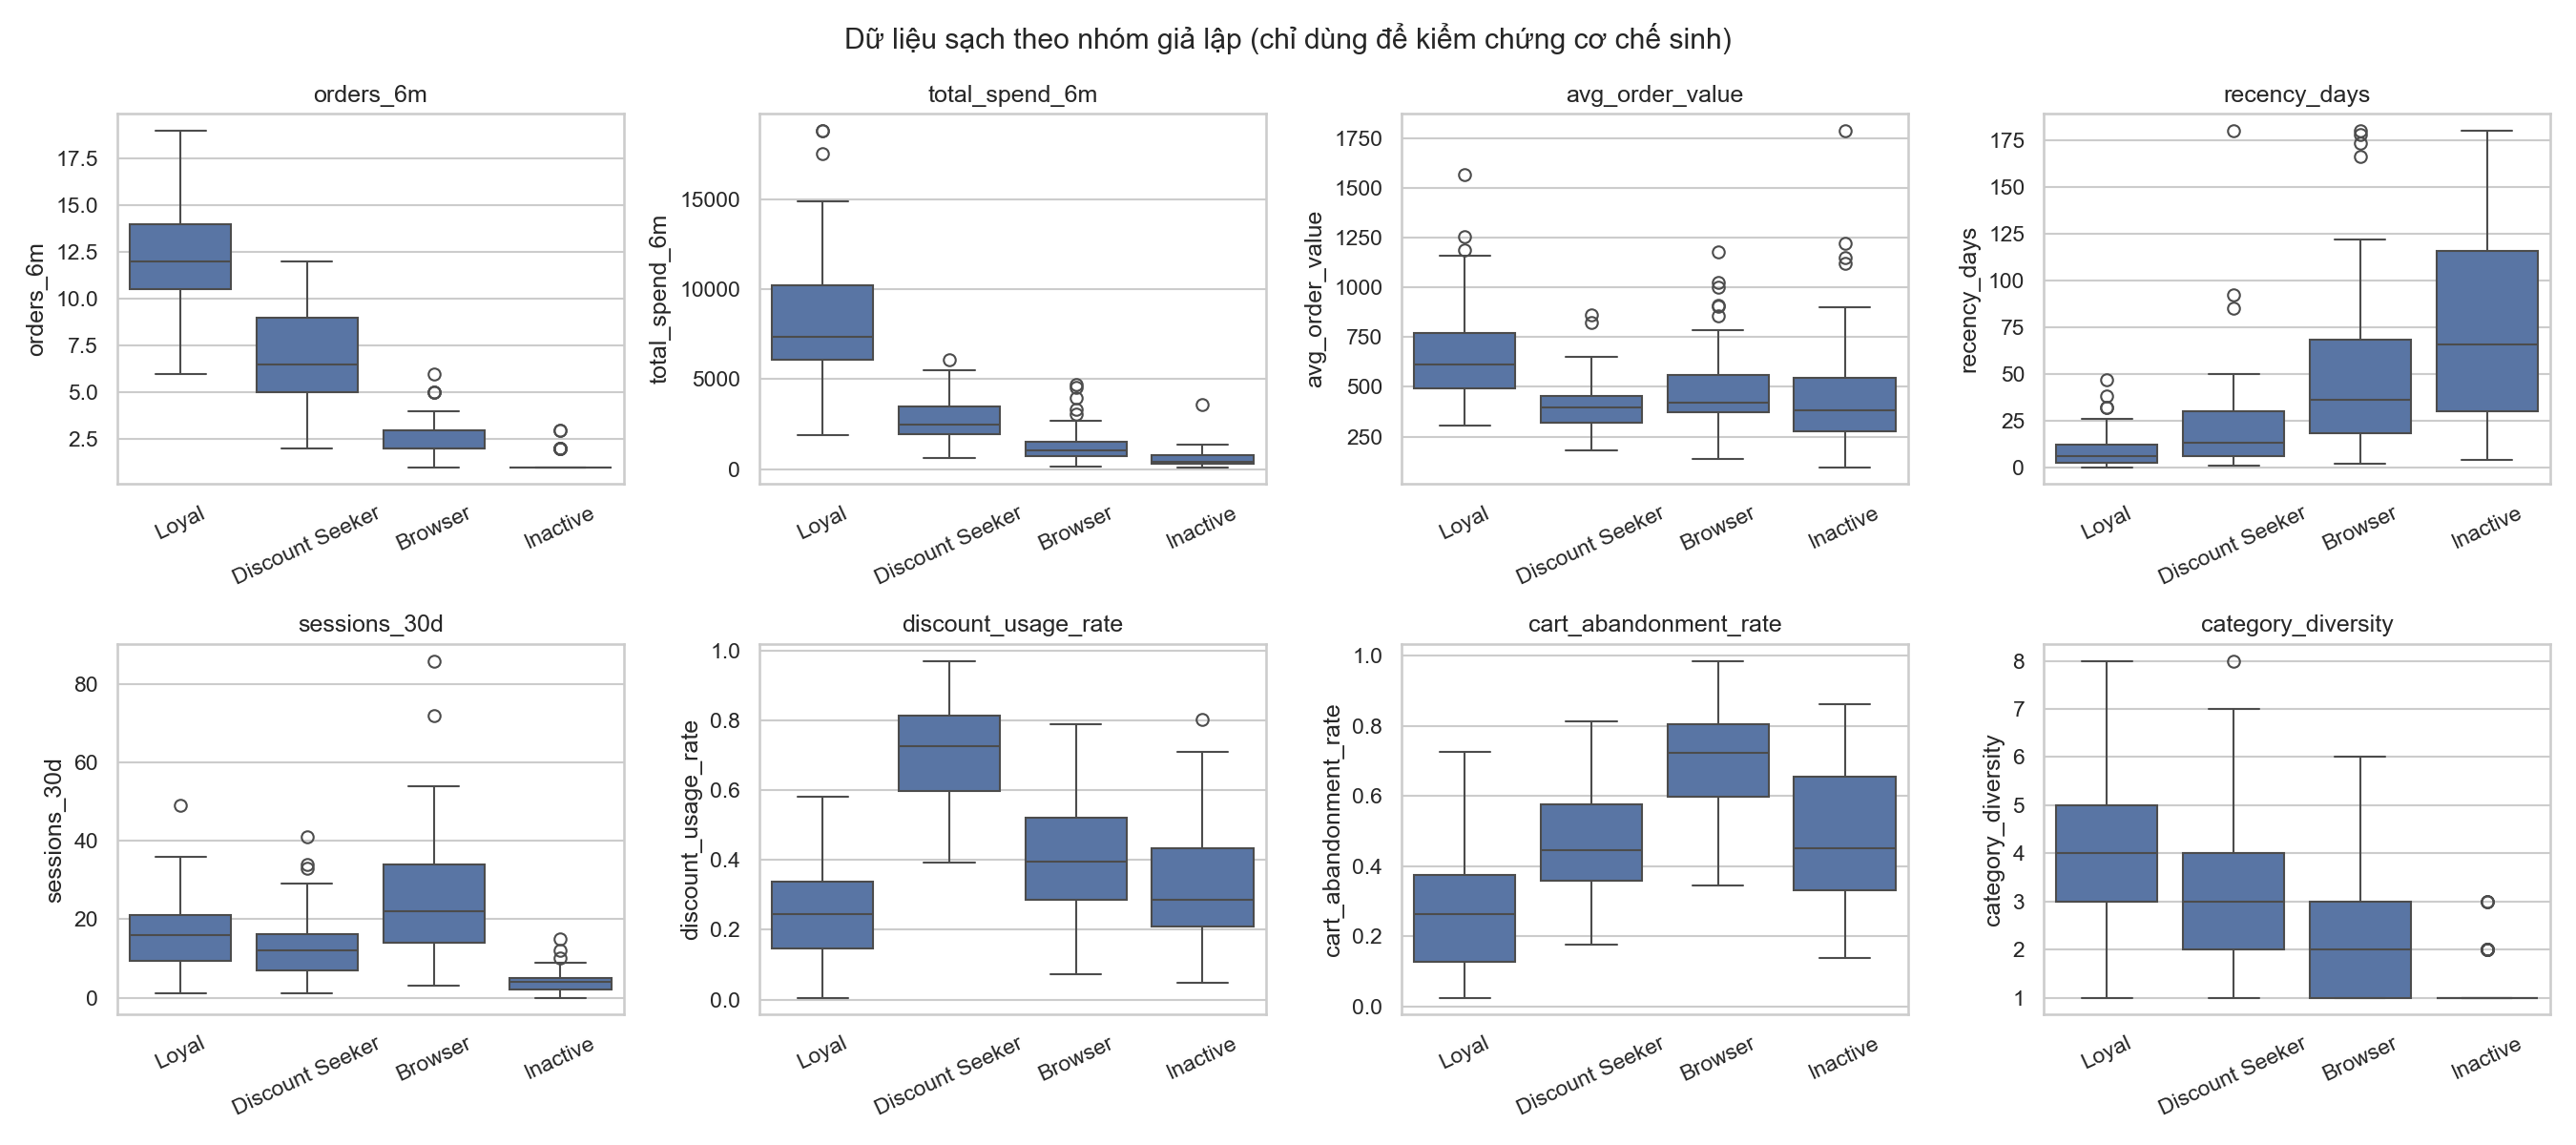
\includegraphics[width=\textwidth]{a_clean_features_by_segment.png}
  \caption{Dữ liệu sạch theo nhóm giả lập (chỉ dùng để kiểm chứng cơ chế sinh).}
  \label{fig:segments}
\end{figure}

%===========================================================================
\section{Câu b — Data Understanding}

\paragraph{Phương pháp.}
EDA trên \texttt{customers\_corrupted.csv}, gồm:
\begin{itemize}
  \item kích thước, kiểu dữ liệu, trùng lặp; thống kê mô tả và skewness; tần suất biến phân loại;
  \item tỷ lệ thiếu và quan hệ của giá trị thiếu với các biến khác;
  \item histogram (thang gốc và log1p); boxplot sau robust z-score $(x - \text{median})/\text{IQR}$;
  \item heatmap Pearson và Spearman; kiểm tra quy tắc nghiệp vụ; phát hiện ngoại lai bằng IQR.
\end{itemize}
Dữ liệu gốc chỉ dùng để so sánh thống kê trước/sau khi đưa vào lỗi; metadata chỉ dùng để đánh giá khả năng phát hiện ngoại lai.

\paragraph{Lý do lựa chọn.}
Robust z-score và Spearman được dùng song song với các thống kê thông thường, vì mean, std và Pearson bị chính các ngoại lai làm sai lệch. Quy tắc nghiệp vụ bắt được giá trị vi phạm miền mà IQR có thể bỏ sót; IQR bắt được giá trị cực lớn vẫn hợp lệ về miền.

\paragraph{Kết quả và nhận xét.}
Không có bản ghi trùng lặp. Có \MissingRecords{} bản ghi (\MissingRecordsPct\%) thiếu ít nhất một giá trị. Bốn vấn đề ảnh hưởng đến K-Means:

\begin{enumerate}[label=\arabic*.]
  \item \textbf{Phân bố lệch và chênh lệch thang đo.}
  Độ lệch chuẩn của \texttt{total\_spend\_6m} là \StdSpendCorrupted, của \texttt{return\_rate} là \StdReturnCorrupted. Skewness của \texttt{sessions\_30d} là \SkewSessions, của \texttt{total\_spend\_6m} là \SkewSpend.
  K-Means dùng khoảng cách Euclid, nên nếu không đưa về cùng thang đo, biến tiền tệ sẽ quyết định toàn bộ khoảng cách. Đuôi dài của biến lệch phải kéo tâm cụm hoặc chiếm riêng một cụm.

  \item \textbf{Tương quan và dư thừa.}
  Spearman giữa \texttt{orders\_6m} và \texttt{total\_spend\_6m} là \SpearOrdersSpend, trong khi Pearson chỉ \PearOrdersSpend{} do ngoại lai. Nhóm biến mua hàng (số đơn, chi tiêu, giá trị đơn, số danh mục, recency) cùng biến thiên với nhau, nên chiều "mức mua hàng" bị tính nhiều lần trong khoảng cách.

  \item \textbf{Giá trị thiếu.}
  Giá trị thiếu của \texttt{cart\_abandonment\_rate} tập trung ở khách ít truy cập: trung vị số phiên là \CartMissSessMedian{} ở nhóm thiếu, so với \CartObsSessMedian{} ở nhóm có giá trị. \texttt{KMeans} không nhận NaN. Xóa bản ghi sẽ làm mất \MissingRecordsPct\% mẫu và lệch về phía khách hoạt động nhiều.

  \item \textbf{Ngoại lai và nhiễu.}
  So với dữ liệu sạch, độ lệch chuẩn tăng \StdRatioSessions{} lần với số phiên và \StdRatioSpend{} lần với chi tiêu. Pearson giữa số đơn và chi tiêu giảm từ \PearOrigOrdersSpend{} xuống \PearOrdersSpend. Ngoại lai làm phồng std, nên chuẩn hóa z-score sẽ nén sự khác biệt giữa các khách bình thường.
\end{enumerate}

Khả năng phát hiện \OutlierIds{} ngoại lai được trình bày ở Bảng~\ref{tab:detection}:
\begin{itemize}
  \item Quy tắc nghiệp vụ bắt đủ \OutlierError{} lỗi mà không đánh dấu nhầm bản ghi nào.
  \item IQR với $k=1.5$ bắt được \DetIqrOneTotal/\OutlierIds{} và đánh dấu nhầm \DetIqrOneFalse{} bản ghi, chủ yếu do đuôi tự nhiên của recency và chi tiêu. Các ngoại lai mà IQR bỏ sót đều là giá trị âm nhỏ, vẫn nằm trong râu.
  \item Kết hợp quy tắc nghiệp vụ với IQR $k=3$ bắt được \DetCombTotal/\OutlierIds.
\end{itemize}

\begin{table}[H]
  \centering\small
  \caption{Khả năng phát hiện ngoại lai trên dữ liệu corrupted (đối chiếu metadata sau khi phát hiện).}
  \label{tab:detection}
  \begin{adjustbox}{max width=\textwidth}\generated{table_detection.tex}\end{adjustbox}
\end{table}

\begin{figure}[H]
  \centering
  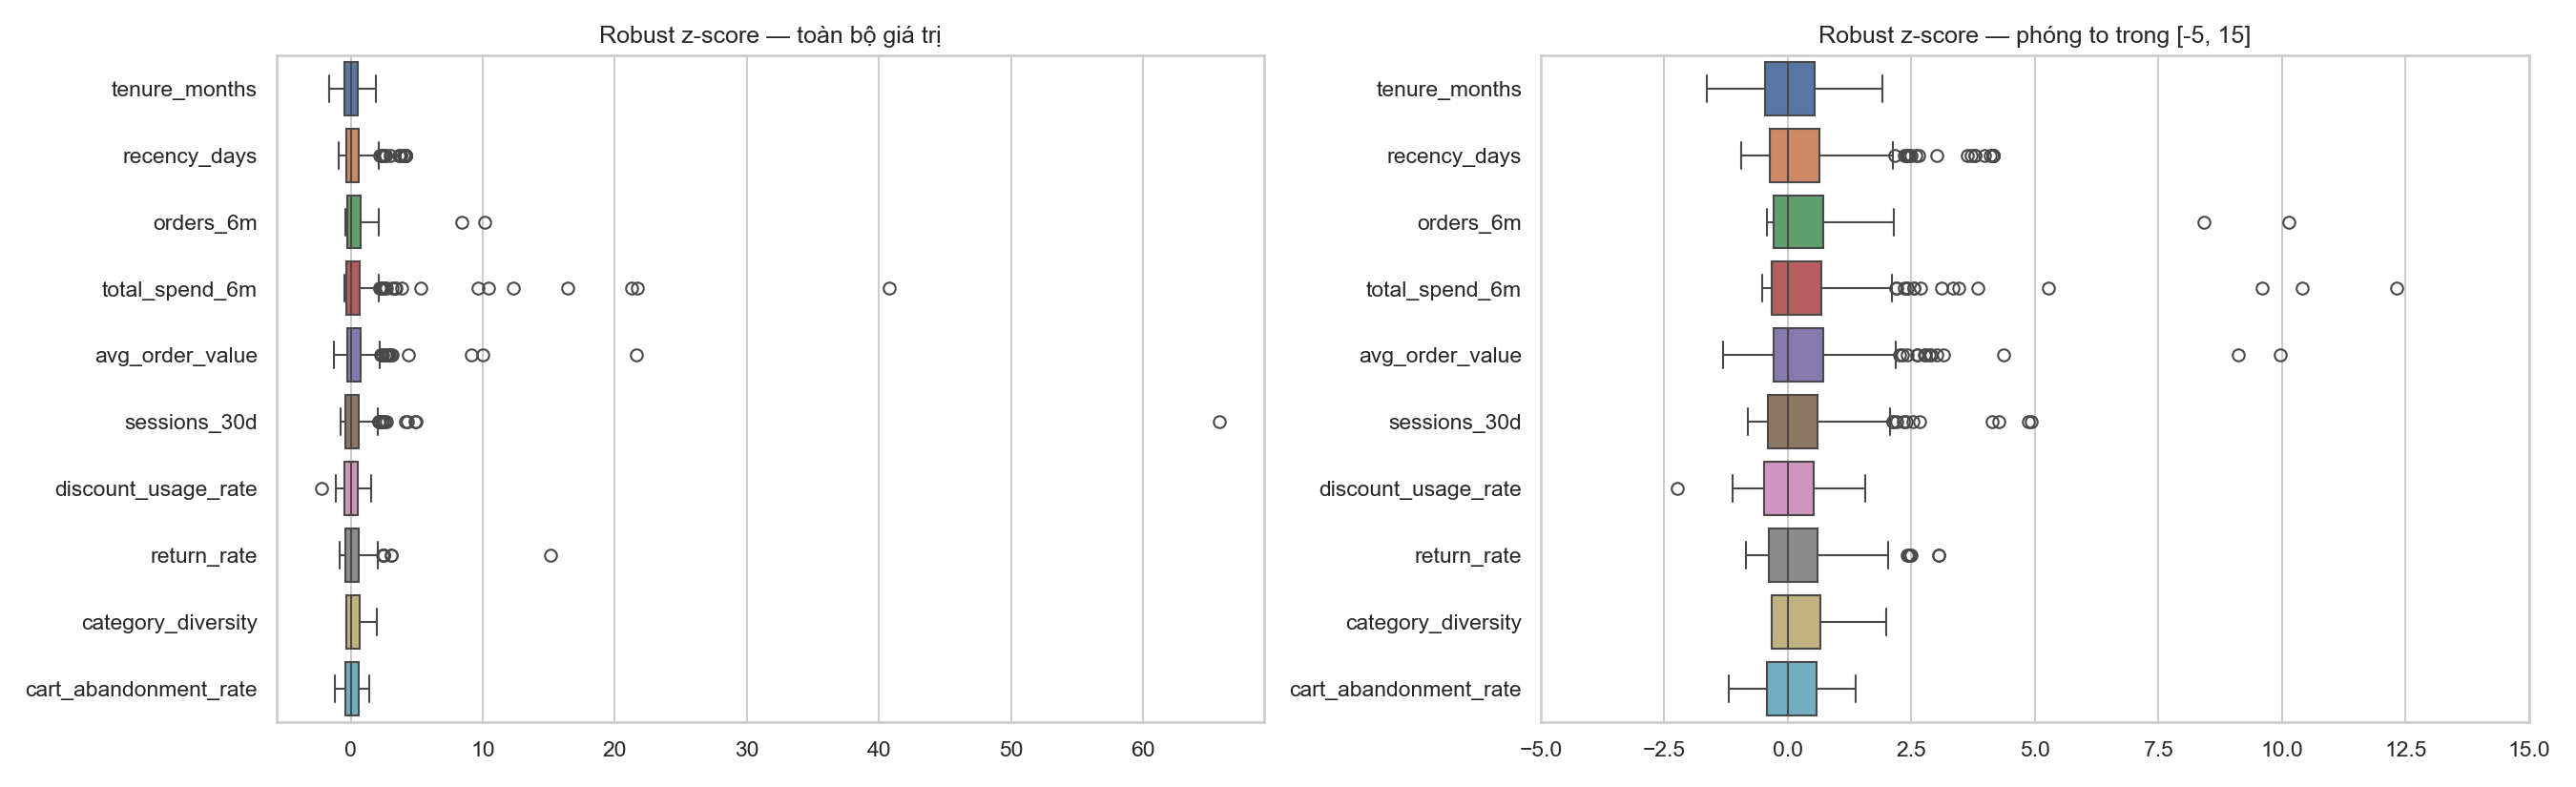
\includegraphics[width=\textwidth]{b_boxplot_robust_scaled.png}
  \caption{Boxplot sau robust z-score trên dữ liệu corrupted.}
\end{figure}

\begin{figure}[H]
  \centering
  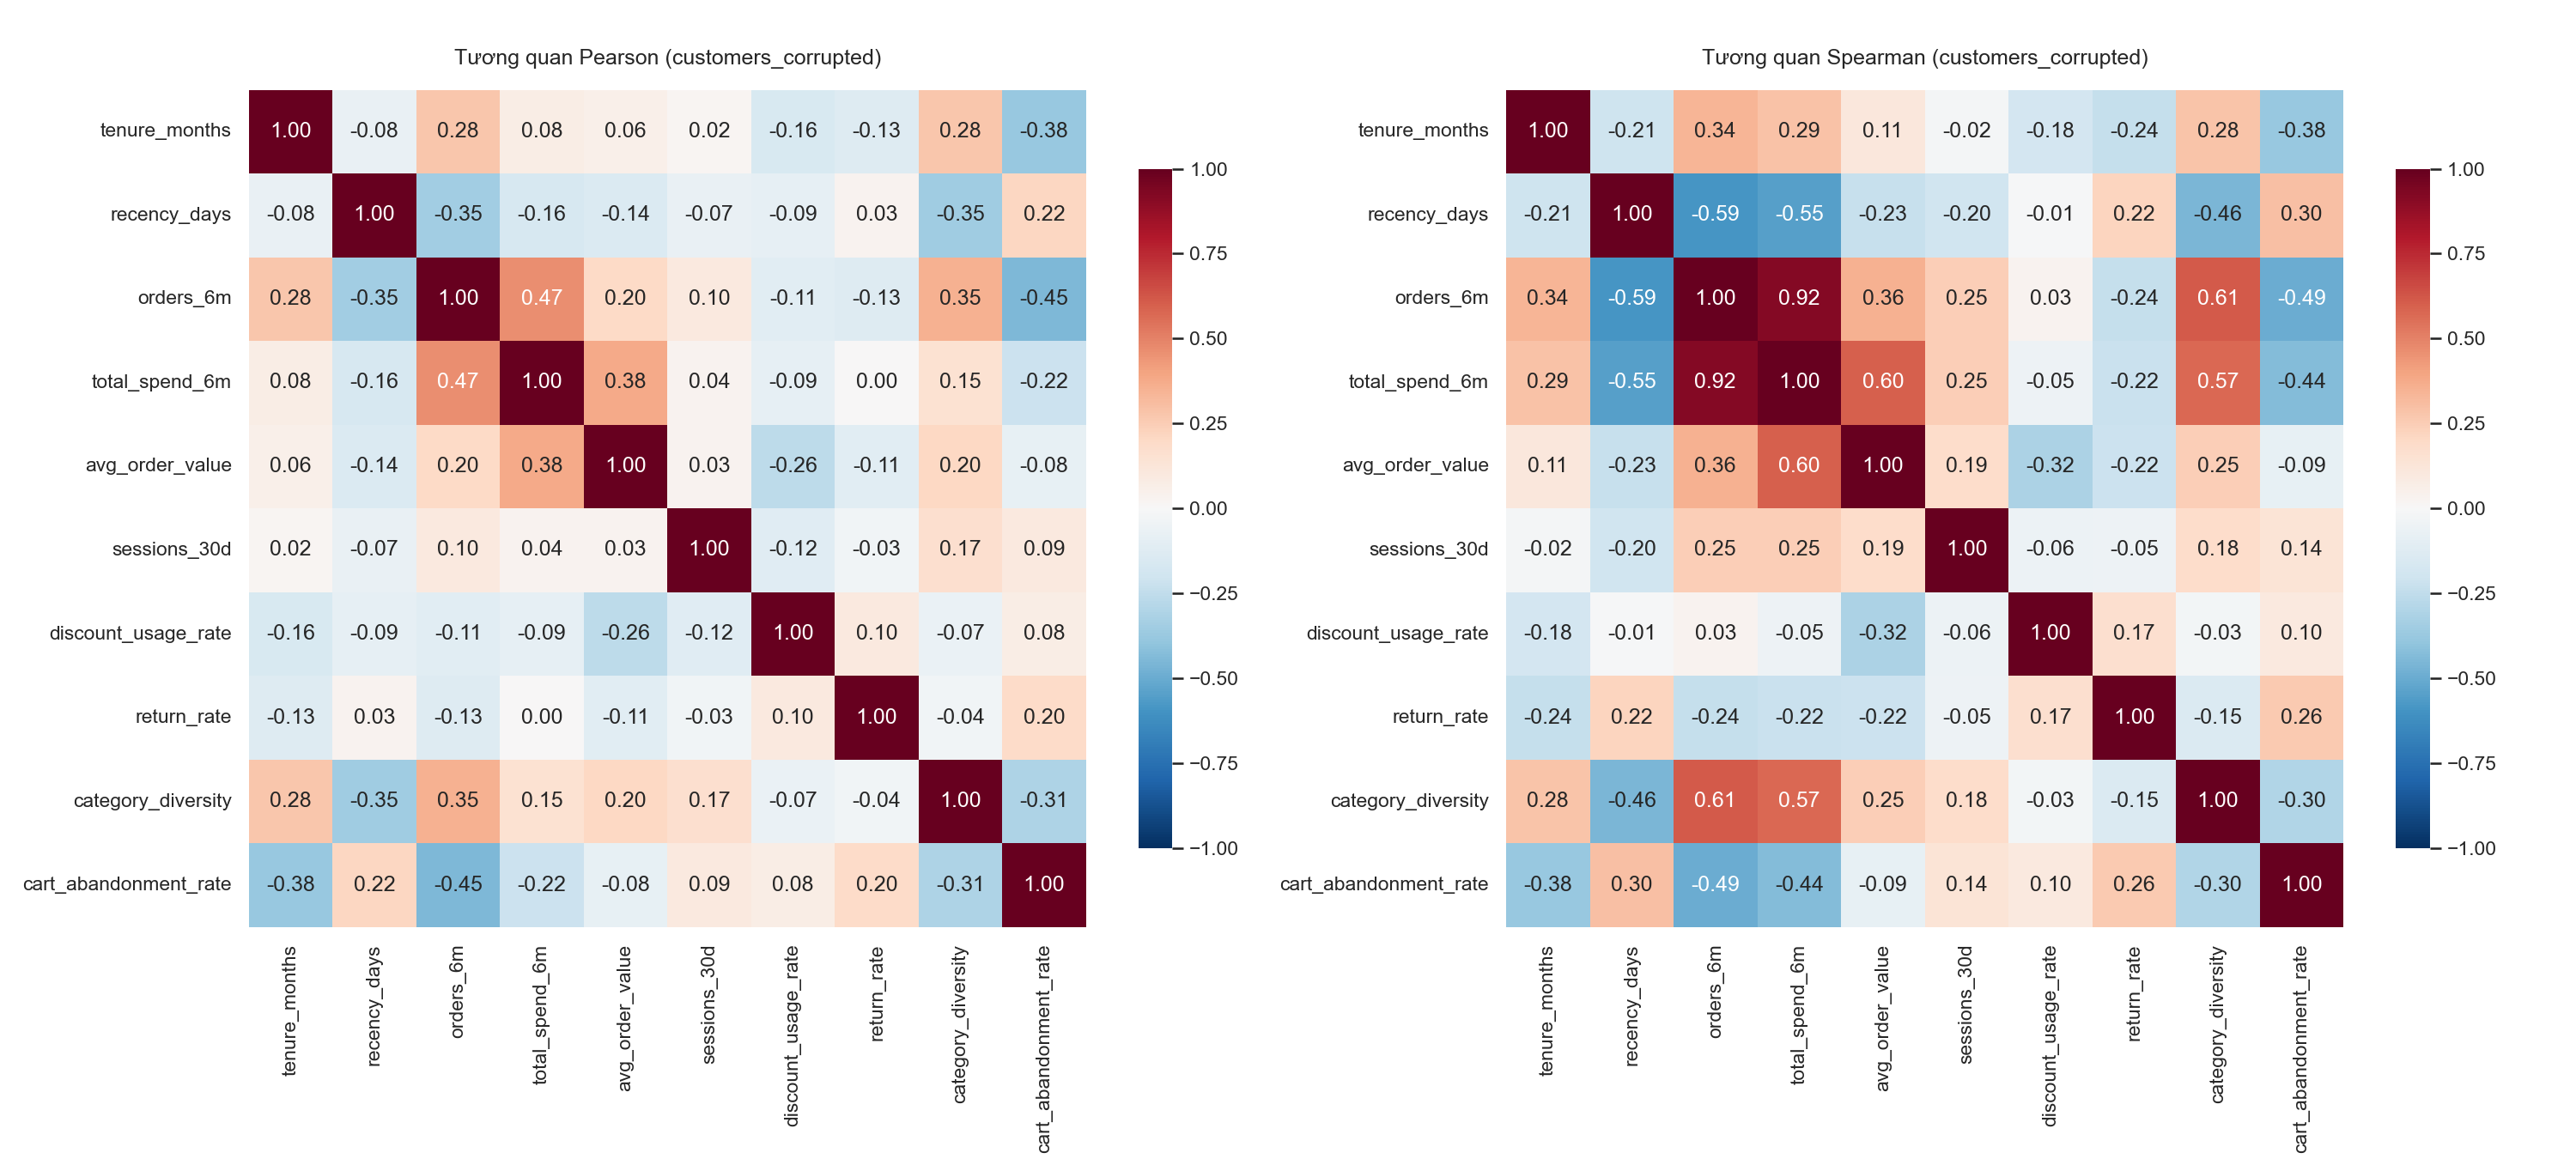
\includegraphics[width=\textwidth]{b_correlation_heatmaps.png}
  \caption{Tương quan Pearson và Spearman trên dữ liệu corrupted.}
\end{figure}

%===========================================================================
\section{Câu c — Data Preprocessing}

\paragraph{Phương pháp.}
Quy trình chỉ dùng \texttt{customers\_corrupted.csv}, gồm bốn bước:
\begin{enumerate}[label=(\arabic*)]
  \item \textbf{Giá trị không hợp lệ $\rightarrow$ NaN} ở mức từng ô: biến đếm hoặc tiền tệ âm; tỷ lệ ngoài $[0,1]$; \texttt{sessions\_30d}~$>300$; \texttt{recency\_days} ngoài cửa sổ quan sát hoặc vượt tenure; $\texttt{total\_spend\_6m}/(\texttt{orders\_6m}\times\texttt{avg\_order\_value})$ ngoài $[0.5, 2]$.
  \item \textbf{Điền khuyết:}
    \begin{itemize}
      \item \texttt{total\_spend\_6m} và \texttt{avg\_order\_value}: theo quan hệ định nghĩa;
      \item \texttt{cart\_abandonment\_rate}: trung vị theo nhóm số đơn (1, 2–3, 4–8, $\ge 9$);
      \item các cột còn lại: trung vị (biến số) hoặc mode (biến phân loại).
    \end{itemize}
  \item \textbf{Phát hiện ngoại lai} bằng IQR trên dữ liệu đã sửa.
  \item \textbf{Xử lý ngoại lai và nhiễu:} không xóa bản ghi; không winsorize khách hợp lệ; không sửa nhiễu.
\end{enumerate}

\paragraph{Lý do lựa chọn.}
\begin{itemize}
  \item Chuyển giá trị sai thành NaN giữ đủ \NCustomers{} bản ghi và chỉ thay đúng ô sai.
  \item Quan hệ định nghĩa dùng thông tin riêng của từng khách, thay vì đặt họ vào giữa phân bố như median imputation.
  \item Trung vị theo nhóm số đơn được chọn vì trên dữ liệu corrupted, \texttt{cart\_abandonment\_rate} tương quan với \texttt{orders\_6m} mạnh hơn nhiều so với \texttt{sessions\_30d}.
  \item Khách chi tiêu hoặc tần suất cao nhưng nhất quán là khách thật. Ảnh hưởng của họ lên khoảng cách được giảm ở câu d bằng biến đổi log: robust z lớn nhất của chi tiêu giảm từ \LogZSpendRaw{} xuống \LogZSpendLog.
  \item Nhiễu Gaussian không tạo giá trị vi phạm quy tắc, nên không thể xác định giá trị nào bị nhiễu khi không biết giá trị thật.
\end{itemize}

\paragraph{Kết quả.}
\begin{itemize}
  \item \InvalidCells{} ô không hợp lệ được chuyển thành NaN, đúng là \OutlierError{} ngoại lai lỗi; không khách VIP nào bị coi là lỗi.
  \item Tổng cộng \ImputedCells{} ô được điều chỉnh, ghi trong \texttt{results/preprocessing\_changes.csv}.
  \item Số ô thiếu giảm từ \MissingCellsBefore{} về 0; không còn bản ghi vi phạm quy tắc.
  \item Độ lệch chuẩn của số phiên giảm từ \SessionsStdBefore{} xuống \SessionsStdAfter; của chi tiêu từ \SpendStdBefore{} xuống \SpendStdAfter.
  \item Sau khi sửa, IQR $k=3$ còn đánh dấu \PreIqrThreeRecords{} bản ghi: \OutlierBusiness{} ngoại lai nghiệp vụ được giữ nguyên, và \PreIqrThreeNotInjected{} bản ghi có giá trị cao tự nhiên.
  \item Còn \SpendRatioDeviating{} bản ghi có chi tiêu lệch hơn 1\% so với tích số đơn và giá trị đơn, tức nhiễu vẫn tồn tại trong dữ liệu.
\end{itemize}

\paragraph{Nhận xét.}
Đánh giá sau xử lý dùng dữ liệu gốc, chỉ để đo, không để chỉnh quy trình:
\begin{itemize}
  \item Điền \texttt{avg\_order\_value} theo định nghĩa cho MAE \MaeAovMethod, so với \MaeAovMedian{} nếu dùng trung vị toàn cục.
  \item Điền \texttt{cart\_abandonment\_rate} theo nhóm số đơn cho MAE \MaeCartMethod, so với \MaeCartMedian{} của trung vị toàn cục. Giả thuyết rằng trung vị có điều kiện chính xác hơn \emph{không được ủng hộ}. Phương pháp vẫn được giữ, vì đã chọn trước khi đánh giá và không kém hơn median imputation.
\end{itemize}

\begin{figure}[H]
  \centering
  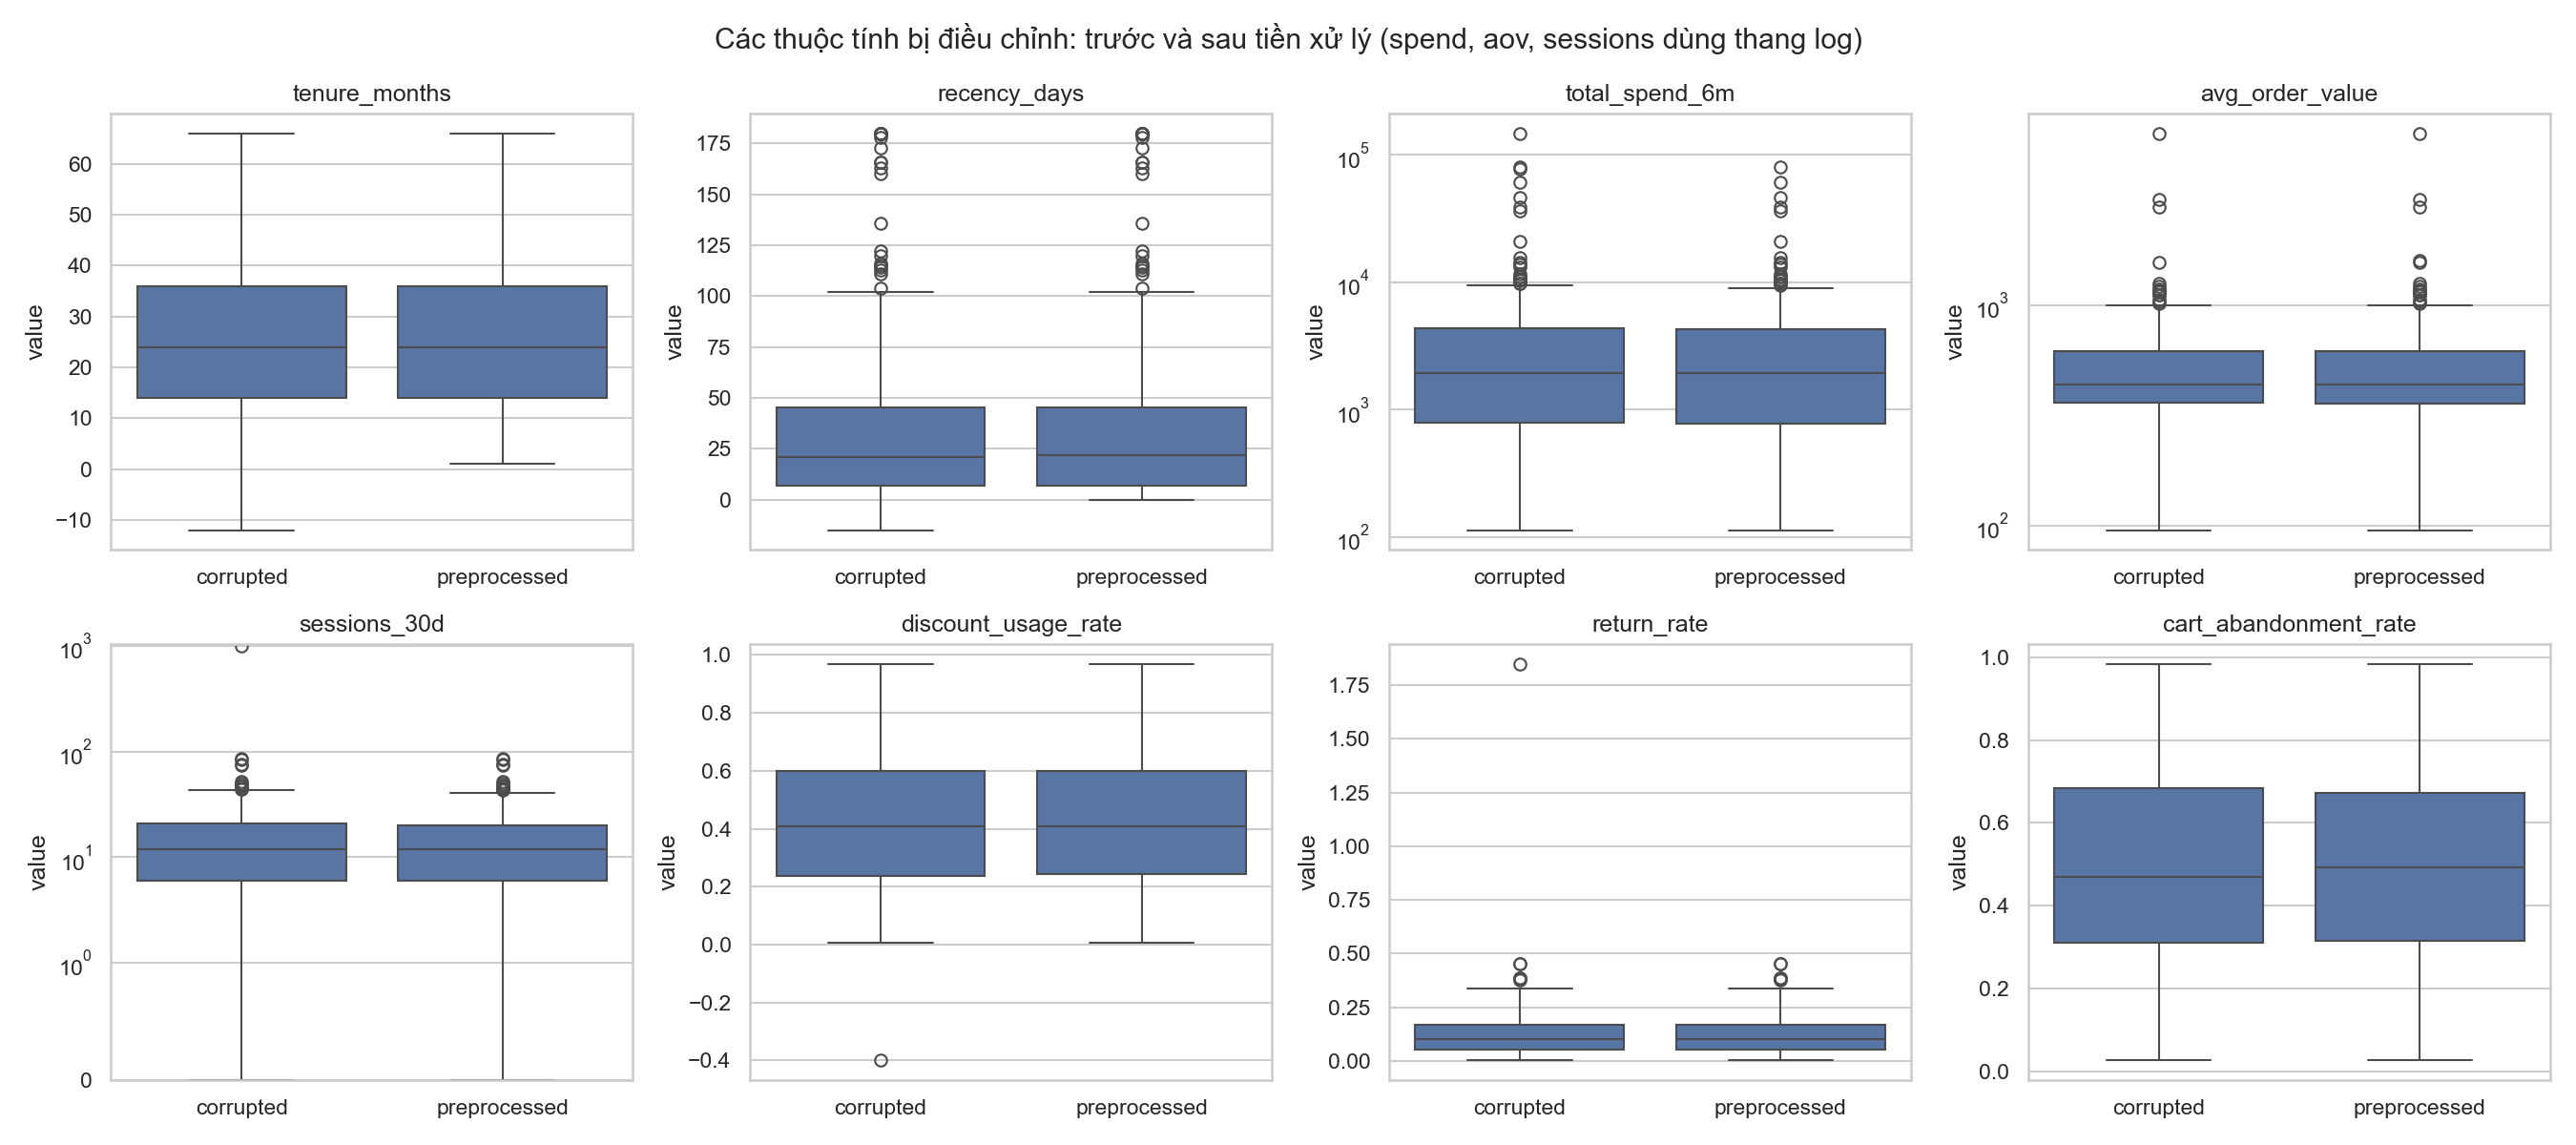
\includegraphics[width=\textwidth]{c_before_after_preprocessing.png}
  \caption{Các thuộc tính bị điều chỉnh trước và sau tiền xử lý.}
\end{figure}

%===========================================================================
\section{Câu d — Data Preparation}

\paragraph{Phương pháp.}
\begin{itemize}
  \item \textbf{Chọn thuộc tính:} loại \texttt{customer\_id}, nhãn và metadata; bỏ \texttt{total\_spend\_6m}.
  \item \textbf{Biến đổi:} log1p cho \texttt{recency\_days}, \texttt{orders\_6m}, \texttt{avg\_order\_value}, \texttt{sessions\_30d}.
  \item \textbf{Chuẩn hóa:} \texttt{RobustScaler} cho \NumericDims{} biến số.
  \item \textbf{Mã hóa:} \texttt{OneHotEncoder} với danh mục cố định cho hai biến phân loại, tạo \OnehotDims{} cột, nhân trọng số $1/\sqrt{2}$.
  \item \textbf{PCA:} chỉ dùng để trực quan hóa.
\end{itemize}

\paragraph{Lý do lựa chọn.}
\begin{itemize}
  \item Trên thang log, $\log(\text{orders}) + \log(\text{aov})$ giải thích \LogSpendExplainedPct\% phương sai của $\log(\text{spend})$. Giữ cả ba sẽ tính thông tin mua hàng hai lần. Hai biến thành phần mang ý nghĩa tách biệt (tần suất và giá trị mỗi lần mua), còn tổng chi tiêu được giữ trong dữ liệu đã tiền xử lý để mô tả cụm.
  \item Các cặp tương quan vừa phải (ví dụ số đơn và số danh mục) được giữ, vì mỗi biến đo một khía cạnh khác nhau.
  \item RobustScaler dùng median và IQR, nên không bị khách VIP và nhiễu còn lại kéo lệch. Nhược điểm là std sau chuẩn hóa không đồng đều: \texttt{log\_avg\_order\_value} chiếm \AovVarSharePct\% tổng phương sai.
  \item Trọng số $1/\sqrt{2}$ khiến một biến phân loại khác mức đóng góp đúng 1 vào bình phương khoảng cách, thay vì 2.
\end{itemize}

\paragraph{Kết quả và nhận xét.}
Ma trận cuối có kích thước $\NCustomers \times \FeatureDims$: $\NInputFeatures - \NDropped + (\NCategories + \NDevices - 2) = \FeatureDims$ chiều. Ma trận không có NaN hay vô cực, và không chứa cột ID hay nhãn; được lưu trong \texttt{data/customers\_prepared.csv}, còn \texttt{customer\_id} lưu riêng trong \texttt{prepared\_customer\_ids.csv}.

Hai thành phần chính đầu tiên giải thích \PcaTwoPct\% phương sai, năm thành phần đầu giải thích \PcaFivePct\%. Trên mặt phẳng 2D không thấy cụm tách rời, phù hợp với thiết kế các nhóm chồng lấn.

\begin{figure}[H]
  \centering
  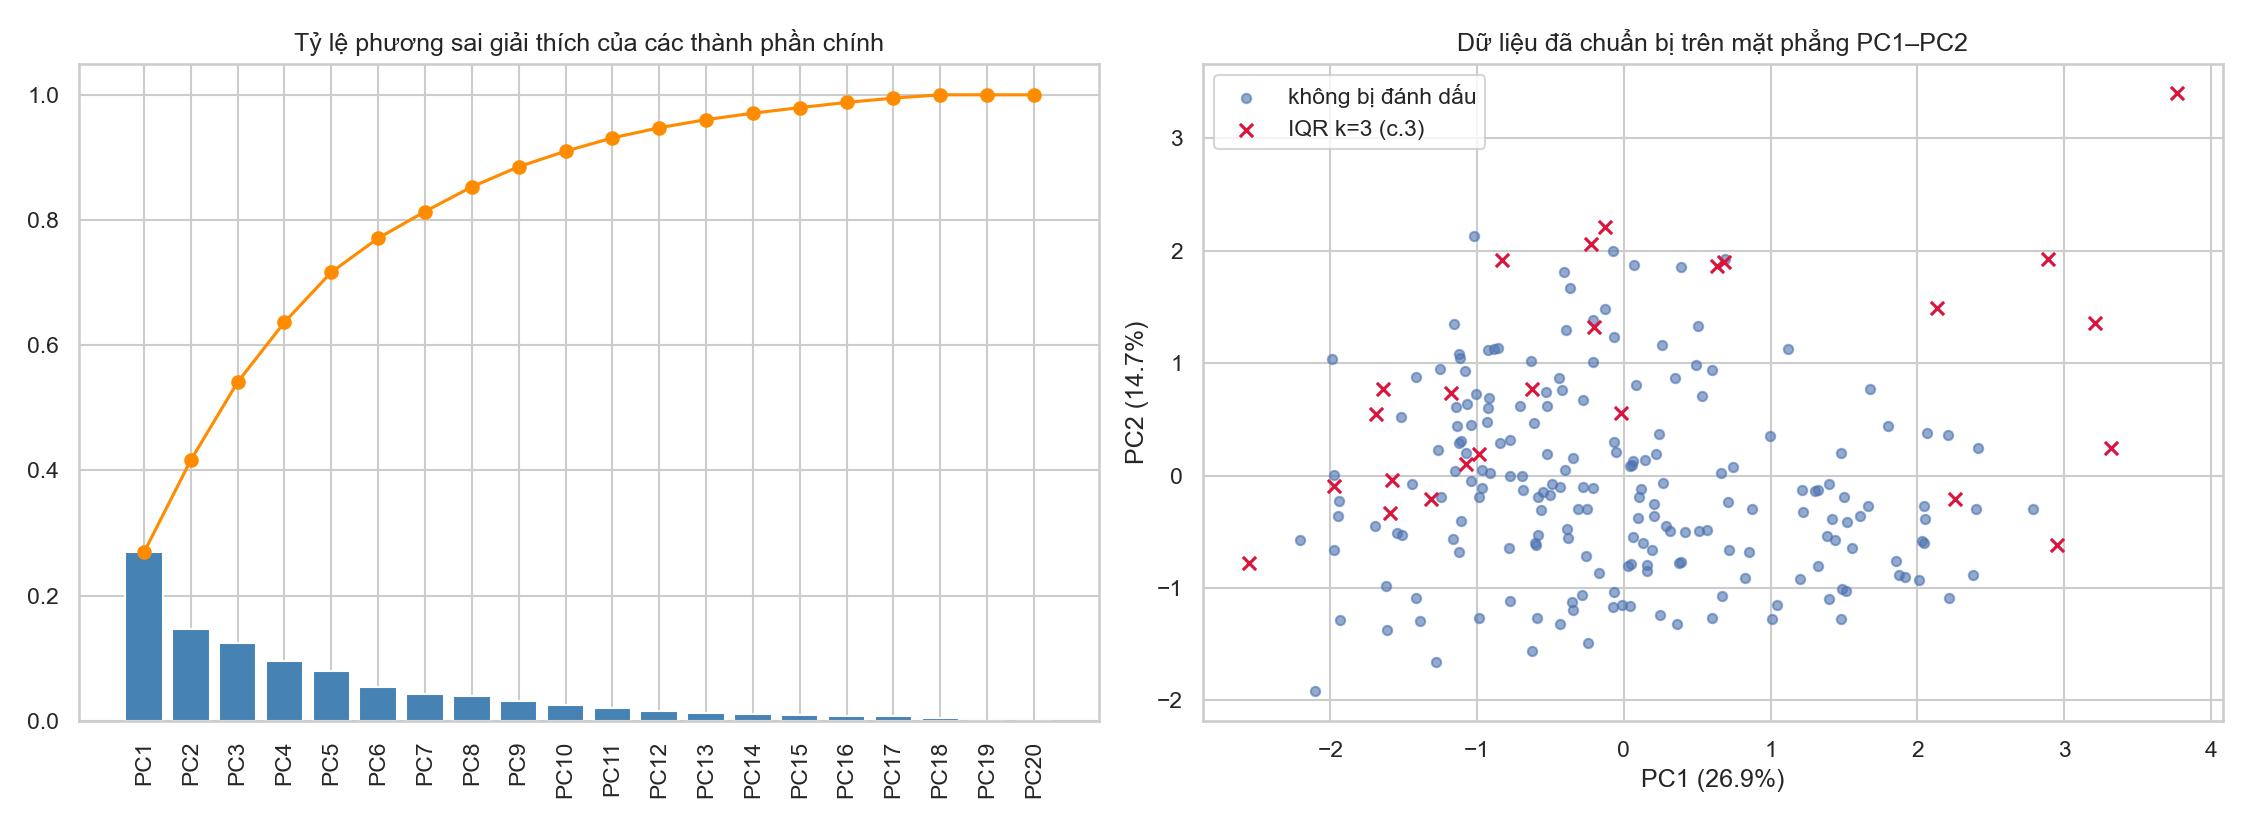
\includegraphics[width=\textwidth]{d_pca_overview.png}
  \caption{Phương sai giải thích và dữ liệu đã chuẩn bị trên mặt phẳng PC1–PC2.}
\end{figure}

%===========================================================================
\section{Câu e — Phân cụm và đánh giá}

\paragraph{Phương pháp.}
K-Means với \texttt{n\_init=20}, \texttt{random\_state=42}, chạy trên hai nhánh:
\begin{itemize}
  \item \textbf{Nhánh A (baseline):} dữ liệu corrupted, chỉ điền trung vị hoặc mode. Phép log1p cắt giá trị âm tại 0 vì hàm log không xác định; các lỗi khác được giữ nguyên.
  \item \textbf{Nhánh B (processed):} dữ liệu sau câu c và câu d.
\end{itemize}
Hai nhánh dùng cùng \FeatureDims{} đặc trưng, cùng thứ tự cột và cùng bộ scaler/encoder (fit một lần, áp dụng cho cả hai).

Số cụm được khảo sát với $k = 2,\dots,8$. Quy tắc đặt trước: chọn $k$ có Silhouette cao nhất trên nhánh B. Thí nghiệm bổ sung dùng $k=4$, lấy từ thiết kế giả lập. ARI với \texttt{true\_segment} chỉ được tính sau khi phân cụm. Ngoài ra có một dòng tham chiếu: dữ liệu gốc sạch đi qua cùng bộ biến đổi.

\paragraph{Lựa chọn $k$.}
Silhouette và Davies–Bouldin của nhánh B cùng tốt nhất ở $k=\KMain$ (Bảng~\ref{tab:ksurvey}); inertia giảm đều, không có điểm gãy rõ, mức giảm chỉ nhỏ lại sau $k=\KDesign$. Ở nhánh A, mọi $k \ge 3$ đều có một cụm chỉ gồm 1 bản ghi (với $k=\KDesign$ là bản ghi có \texttt{return\_rate}~$>1$), khiến Silhouette và Davies–Bouldin của A đẹp bất thường ở $k=3$. Nếu chọn $k$ theo baseline, lựa chọn sẽ bị lỗi dữ liệu chi phối.

\begin{table}[H]
  \centering\small
  \caption{Khảo sát số cụm (Sil.: Silhouette; DB: Davies–Bouldin).}
  \label{tab:ksurvey}
  \begin{adjustbox}{max width=\textwidth}\generated{table_k_survey.tex}\end{adjustbox}
\end{table}

\begin{table}[H]
  \centering\small
  \caption{Kết quả phân cụm của hai nhánh và tham chiếu dữ liệu sạch.}
  \label{tab:metrics}
  \begin{adjustbox}{max width=\textwidth}\generated{table_metrics.tex}\end{adjustbox}
\end{table}

\paragraph{Kết quả và nhận xét.}
\begin{itemize}
  \item \textbf{Thực nghiệm chính ($k=\KMain$).} Nhánh B tốt hơn A ở cả ba chỉ số nhưng mức chênh nhỏ: Silhouette \SilMainA{} lên \SilMainB, Davies–Bouldin \DbMainA{} xuống \DbMainB, ARI \AriMainA{} lên \AriMainB. ARI giữa hai cách gán cụm là \AriAvsBMain. Ranh giới chính là mức độ mua hàng, đủ rõ để các lỗi dữ liệu không làm thay đổi đáng kể.
  \item \textbf{Thí nghiệm bổ sung ($k=4$).}
    \begin{itemize}
      \item Tiền xử lý loại bỏ cụm 1 phần tử: kích thước cụm từ \SizesKfourA{} thành \SizesKfourB.
      \item ARI tăng từ \AriKfourA{} lên \AriKfourB. Mức tương đồng với kết quả trên dữ liệu sạch tăng từ \AriAvsCleanKfour{} lên \AriBvsCleanKfour.
      \item Davies–Bouldin lại xấu hơn (\DbKfourA{} so với \DbKfourB), vì cụm 1 phần tử có độ phân tán bằng 0 và nằm xa, nên kéo chỉ số trung bình của A xuống. Giá trị của B gần với tham chiếu sạch (\DbKfourClean).
      \item Các chỉ số dựa trên khoảng cách có thể ``thưởng'' cho việc tách riêng một điểm lỗi, nên cần đọc cùng với kích thước cụm và ý nghĩa nghiệp vụ.
    \end{itemize}
\end{itemize}

\begin{figure}[H]
  \centering
  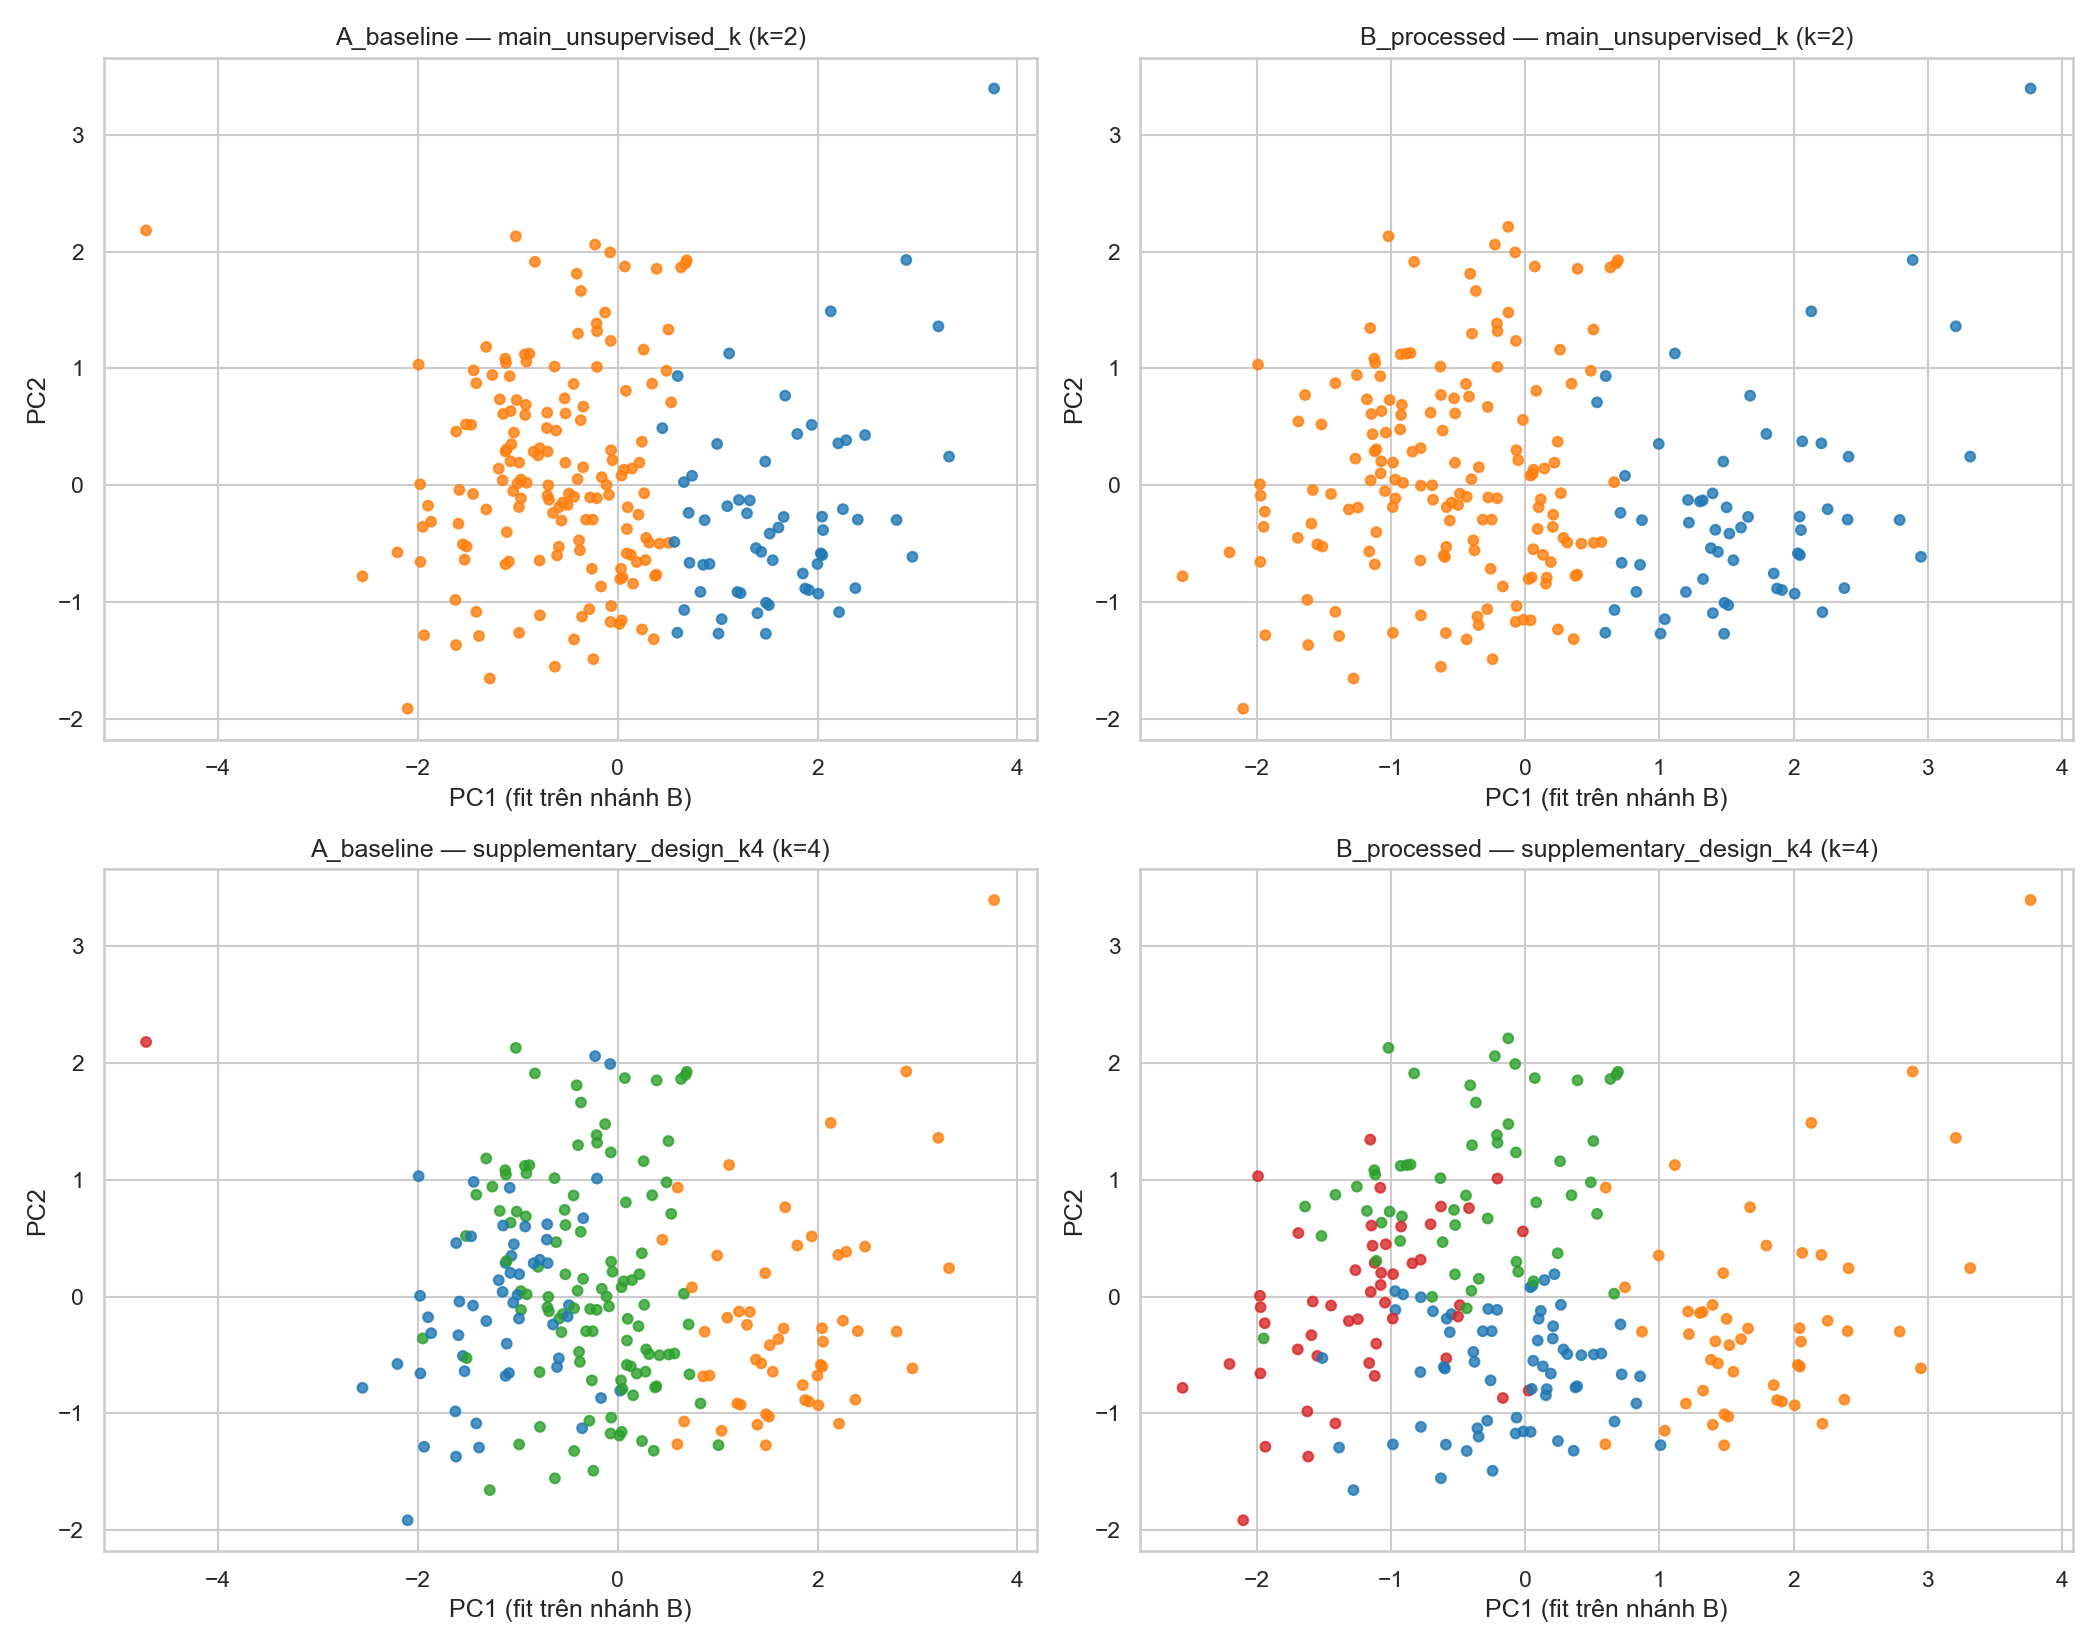
\includegraphics[width=0.85\textwidth]{e_clusters_pca.png}
  \caption{Cụm của hai nhánh trên cùng mặt phẳng PCA (fit trên nhánh B).}
\end{figure}

\paragraph{Phân tích cụm.}
Hồ sơ cụm được tính trên dữ liệu nghiệp vụ đã tiền xử lý, không dùng giá trị chuẩn hóa (Bảng~\ref{tab:k2}, \ref{tab:k4}). Tên cụm đặt theo hành vi của các thành viên.

Với $k=\KMain$, cụm thứ hai gộp các kiểu khách cần cách tiếp cận khác nhau, nên phân chia này quá thô cho tiếp thị. Với $k=\KDesign$, bốn cụm có ý nghĩa hành động rõ ràng hơn.

Ở nhánh A, hồ sơ cụm bị lỗi làm méo: hai lỗi chi tiêu $\times 100$ và giá trị 999 phiên làm tăng giá trị trung bình của cụm chứa chúng. Lỗi trong \texttt{total\_spend\_6m} không ảnh hưởng việc gán cụm (vì cột này không nằm trong tập đặc trưng), nhưng làm sai thông tin dùng để ra quyết định.

\begin{table}[H]
  \centering\small
  \caption{Hồ sơ cụm nhánh B, $k=\KMain$ (tiền: nghìn đồng; giảm giá, bỏ giỏ: tỷ lệ trung bình).}
  \label{tab:k2}
  \begin{adjustbox}{max width=\textwidth}\generated{table_profiles_B_main.tex}\end{adjustbox}
\end{table}

\begin{table}[H]
  \centering\small
  \caption{Hồ sơ cụm nhánh B, $k=4$.}
  \label{tab:k4}
  \begin{adjustbox}{max width=\textwidth}\generated{table_profiles_B_k4.tex}\end{adjustbox}
\end{table}

\begin{figure}[H]
  \centering
  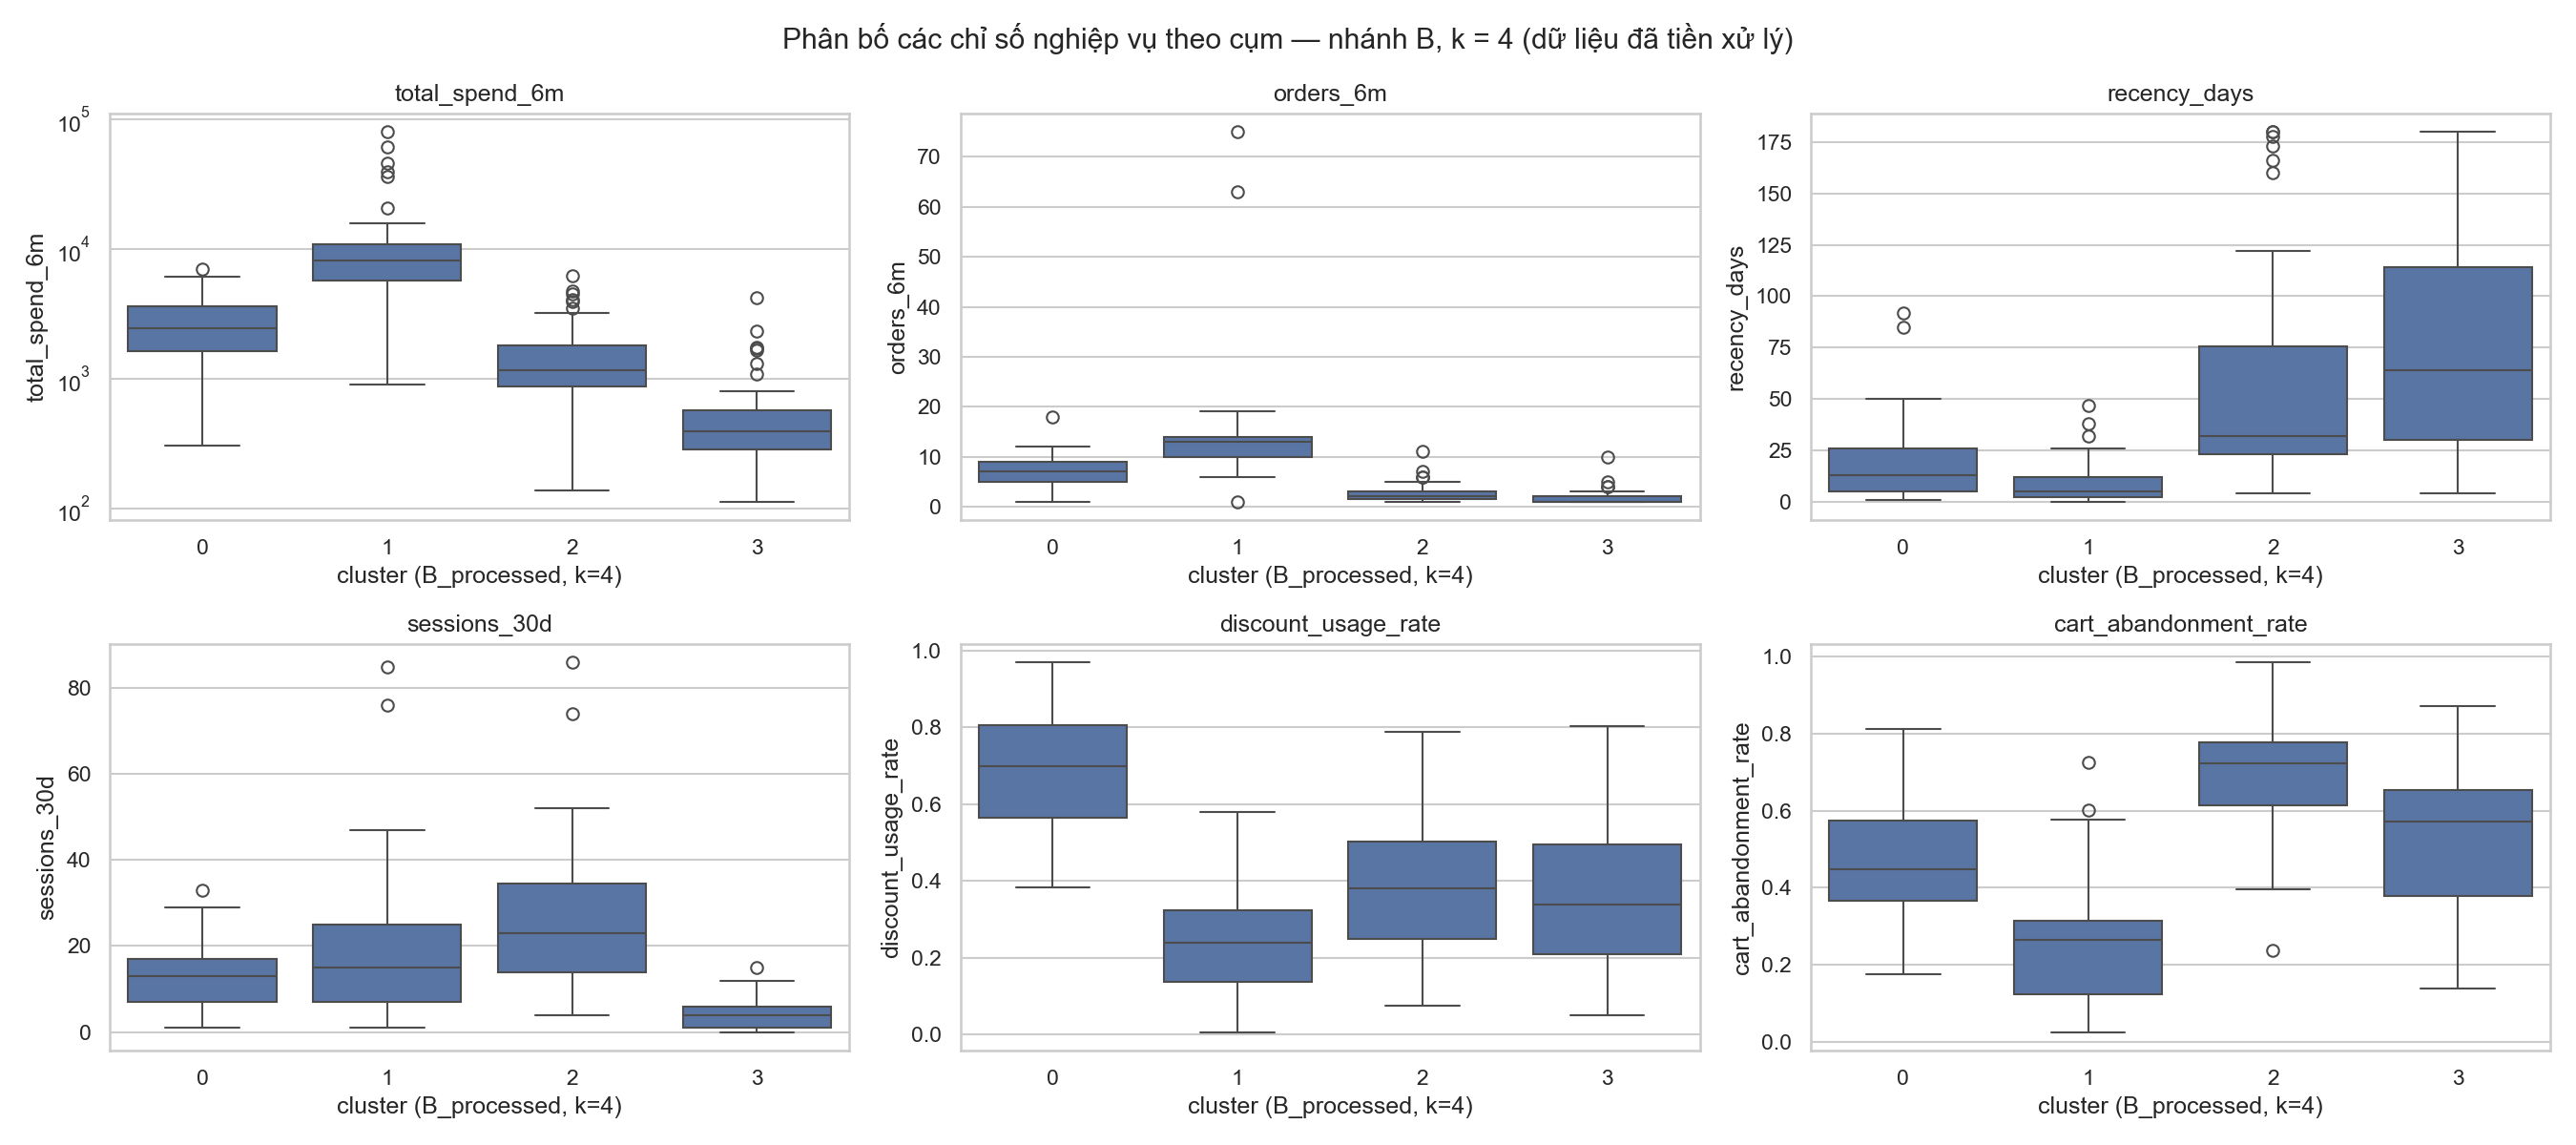
\includegraphics[width=\textwidth]{e_cluster_profiles_B_k4.png}
  \caption{Phân bố các chỉ số nghiệp vụ theo cụm, nhánh B, $k=4$.}
\end{figure}

\paragraph{Đề xuất tiếp thị (bốn cụm của nhánh B).}
\begin{itemize}
  \item \textbf{Trung thành giá trị cao:} hạng thành viên, ưu đãi độc quyền, bán chéo sản phẩm cao cấp. Hạn chế mã giảm giá đại trà, vì nhóm này ít dùng giảm giá.
  \item \textbf{Săn khuyến mãi:} voucher có mục tiêu, flash sale, combo hoặc ngưỡng miễn phí vận chuyển để tăng giá trị đơn. Cần theo dõi biên lợi nhuận.
  \item \textbf{Xem nhiều, ít mua:} nhắc giỏ hàng bị bỏ, retargeting, thông báo giảm giá sản phẩm đã xem, đơn giản hóa thanh toán.
  \item \textbf{Ít hoạt động:} chiến dịch kích hoạt lại chi phí thấp, khảo sát lý do; ngân sách giới hạn theo giá trị kỳ vọng.
\end{itemize}

Tiêu chí không giám sát ưu tiên $k=\KMain$. Việc dùng $k=4$ cho tiếp thị dựa trên khả năng diễn giải nghiệp vụ. ARI cao hơn chỉ là xác nhận sau nhờ có nhãn giả lập; dữ liệu thực sẽ không có thông tin này.

%===========================================================================
\section{Kết luận}

Tác động của từng vấn đề dữ liệu và của tiền xử lý:
\begin{itemize}
  \item \textbf{Giá trị thiếu} chặn K-Means chạy trực tiếp. Điền trung vị toàn cục ở baseline còn tạo thêm mâu thuẫn giữa các trường của cùng một khách. Điền theo quan hệ định nghĩa giảm mạnh sai số với \texttt{avg\_order\_value}. Điền theo nhóm không cải thiện được \texttt{cart\_abandonment\_rate}.
  \item \textbf{Nhiễu} làm mờ ranh giới giữa các cụm vốn đã chồng lấn và không thể loại bỏ khi không biết giá trị thật. Quy trình chỉ hạn chế ảnh hưởng của nhiễu bằng thống kê bền vững và biến đổi log.
  \item \textbf{Ngoại lai lỗi} có tác động lớn nhất: một bản ghi đủ để chiếm riêng một cụm, làm lệch lựa chọn $k$ và làm méo hồ sơ cụm. Quy tắc nghiệp vụ phát hiện và sửa được toàn bộ \OutlierError{} lỗi.
  \item \textbf{Ngoại lai hợp lệ} được giữ lại; biến đổi log và RobustScaler đủ để chúng không tạo cụm riêng.
  \item \textbf{Tiền xử lý} cải thiện nhẹ ở $k=\KMain$ và cải thiện rõ ở $k=4$ (ARI \AriKfourA{} lên \AriKfourB), qua đó ủng hộ giả thuyết ban đầu. Tuy vậy, không phải chỉ số khoảng cách nào cũng cải thiện theo cùng hướng.
\end{itemize}

\paragraph{Hạn chế.}
\begin{itemize}
  \item Dữ liệu là giả lập: cấu trúc bốn nhóm, tham số phân phối và cơ chế lỗi do người thiết kế chọn, nên các kết quả phản ánh giả định của mô phỏng.
  \item Mẫu nhỏ (\NCustomers{} bản ghi): các chỉ số có phương sai lớn, kết quả có thể khác với seed khác. Cơ chế thiếu khó xác định từ dữ liệu: biến MCAR vẫn cho khác biệt quan sát được giữa nhóm thiếu và nhóm có giá trị.
  \item Mỗi ngoại lai được tạo chỉ mang một loại lỗi, không chồng với nhiễu hay giá trị thiếu, đơn giản hơn dữ liệu thực.
  \item K-Means giả định cụm dạng cầu, kích thước tương đương, và nhạy với thang đo, trọng số đặc trưng (ví dụ tỷ trọng lớn của \texttt{log\_avg\_order\_value}) và ngoại lai. Silhouette của mọi cấu hình đều thấp.
  \item Kết luận chưa được kiểm chứng trên dữ liệu thực; các quy tắc nghiệp vụ và ngưỡng (ví dụ 300 phiên, tỷ lệ chi tiêu $[0.5, 2]$) cần được hiệu chỉnh theo nền tảng cụ thể.
\end{itemize}

%===========================================================================
\section{Kiểm chứng pipeline}

Mỗi điều kiện kiểm chứng bắt buộc được viết thành một hàm kiểm tra trong notebook và đều đạt (Bảng~\ref{tab:checks}). Kiểm tra số 11 chạy lại toàn bộ bước sinh dữ liệu với một bộ sinh mới cùng seed và so khớp với các tệp đã lưu. Kiểm tra số 12 đối chiếu các macro dùng trong báo cáo này với các tệp kết quả CSV.

\begin{table}[H]
  \centering\small
  \caption{Kết quả kiểm chứng tự động.}
  \label{tab:checks}
  \begin{adjustbox}{max width=\textwidth}\generated{table_pipeline_checks.tex}\end{adjustbox}
\end{table}

%===========================================================================
\section{Khai báo sử dụng AI và công cụ}

Bài làm có sử dụng trợ lý AI \textbf{Claude Code} (Anthropic), chạy trong tiện ích VS Code, với mô hình Claude Sonnet 5.5 ở đầu phiên và Claude Opus 5.5 trong phần lớn quá trình thực hiện. AI hỗ trợ: viết và chạy mã Python trong notebook, sửa lỗi phát sinh khi chạy, soạn nhận xét dựa trên kết quả đã chạy, soạn báo cáo này, và rà soát mã. Sinh viên cung cấp đề bài, các ràng buộc thực hiện, và quyết định các lựa chọn được hỏi trong quá trình làm.

Mọi số liệu trong báo cáo được sinh tự động từ kết quả chạy notebook. Các kết quả trái kỳ vọng được giữ nguyên và giải thích. Lịch sử hội thoại chính, các công cụ và phiên bổ sung được khai báo chi tiết trong tệp riêng \texttt{reports/ai\_declaration.tex}.

\end{document}
